\subsubsection{Volume Rendering:}
\label{sec:vr}

Volume rendering is the process of converting a 3D set of data and rendering to the screen.
There are two types of volume rendering ray-casting, and slice-based.
This section will look at the first type of volume rendering.
This type of ray casting is done by drawing a ray from the eye position through the 3D object and then calculating the colour of the object by blending the data found whilst iterating through the ray.
Figure \ref{fig:ray_casting2} shows an example of rays being caste from the camera position through the 3D volume.

\begin{figure}[ht!]
	\centering
	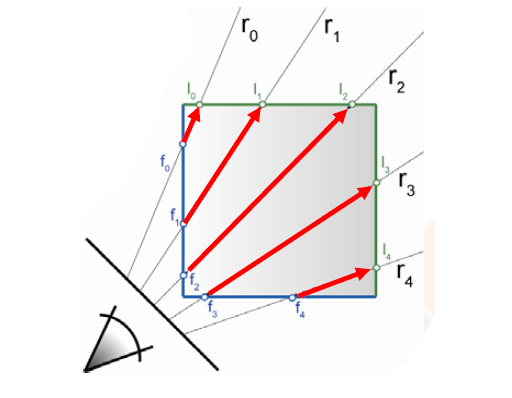
\includegraphics[width=90mm]{images/ray_thumb.PNG}
	\caption{\cite{KHayward09} - Volume Ray Casting}
	\label{fig:ray_casting2}
\end{figure}

This process is very simple and is used only to draw the 3D object in the world and doesn't take in any of the computationally heavy natural phenomenon that happens to light passing through a cloud.